\section{Vibe-Coding Fault Taxonomy}

Vibe coding is not a mood. It is a fault class: shipping code whose correctness depends on plausibility, confidence, or reviewer intuition instead of machine-checkable proof. The risk-priority number below is \textbf{RPN = impact $\times$ likelihood $\times$ detection difficulty}. It is a humanlint policy weight, not a universal incident statistic. Future releases should calibrate it against repair success, escaped defects, security regressions, and review time.

Public evidence supports treating vibe coding as a high-risk production pattern rather than a harmless workflow style. Veracode reports that AI-generated samples introduced risky security flaws in 45\% of tests \cite{veracodeGenaiCodeSecurity2025}. GitGuardian reports accelerating hardcoded-secret exposure in public GitHub activity and AI-service leak growth \cite{gitguardianSecretsSprawl2026,gitguardianSecretsSprawl2026Blog}. Stack Overflow's 2025 survey reports that developers' largest AI frustration is output that is almost right but not quite, with time-consuming AI-code debugging close behind \cite{stackOverflowAISurvey2025}. OWASP's LLM Top 10 names prompt injection, sensitive information disclosure, supply-chain risk, improper output handling, and excessive agency as first-order AI application risks \cite{owaspLlmTopTen2025}. SetupBench and ContextBench add the operational failure modes: agents still struggle with environment bootstrap and useful context retrieval \cite{setupBench2025,contextBench2026}.

\begin{table*}[t]
\caption{Ranked vibe-coding fault taxonomy. RPN is a humanlint policy priority, not an empirical frequency claim.}
\label{tab:fault-taxonomy}
\centering
\scriptsize
\begin{tabularx}{\textwidth}{L{0.13\textwidth} L{0.05\textwidth} L{0.17\textwidth} Y Y}
\toprule
\textbf{TLR} & \textbf{RPN} & \textbf{Fault} & \textbf{Why it happens} & \textbf{Required control} \\
\midrule
Business truth & 125 & False-green business logic & Code compiles and tests pass, but the product rule is wrong or asserted at the wrong level. & Domain invariants, property tests, golden workflows, DB constraints, incident replay tests. \\
Business truth & 100 & Authorization or data-isolation drift & Agent patches authz in UI, handler, or Python because it is locally easy. & Role matrix tests, negative authz tests, owner-map routing, RLS where useful. \\
Security & 80 & Plausible insecure generated code & Output looks idiomatic while hiding injection, XSS, unsafe deserialization, weak crypto, or logging flaws. & Security lane, SAST/SCA, secure-code rules, threat-model checklist, negative tests. \\
Security & 80 & Secrets and identity sprawl & Credentials leak through code, logs, prompts, fixtures, MCP/tool config, or copied examples. & Push protection, local/CI secret scans, redacted logs, credential inventory, transcript/artifact scan. \\
Security & 75 & Excessive agent agency & Broad terminal, browser, network, or filesystem permissions let agents take unsafe actions. & Least-privilege profiles, destructive-command gates, workspace-only writes, permission receipts. \\
Security & 75 & Prompt injection and hostile context & Issues, docs, pages, or comments ask the model to bypass trusted policy. & Source-trust hierarchy, untrusted-content isolation, tool-call validation, no secrets in context. \\
Verification & 64 & False-green tests & Agent writes tests that prove its implementation rather than the requirement. & Reviewer-owned acceptance criteria, mutation/fault checks, semantic assertions, no snapshot-only proof. \\
Context & 64 & Context retrieval failure & Agent over-reads, under-reads, or follows stale nearby patterns instead of the owner path. & Short root router, owner/test maps, local rules, symbol search, command-output filtering. \\
Contracts & 60 & Contract and DTO drift & Handwritten API types, local fetch wrappers, and stale clients become private contracts. & Generated clients only, contract drift lane, generated-zone lock, compatibility tests. \\
Contracts & 60 & Wrong-layer persistence & UI, API edge, scripts, or Python gain durable truth and bypass application/database policy. & DB access policy, adapters-only SQL, migration and constraint tests, forbidden imports. \\
Context & 48 & Environment/setup hallucination & Unclear setup leads agents to install random tools, change config, or skip DB/service proof. & One-command setup, pinned toolchain, devcontainer where useful, setup proof lane. \\
Verification & 48 & Pixel/UI regression & UI functions while layout, hierarchy, responsive state, overflow, or design tokens break. & Storybook states, Playwright screenshots, geometry rules, baseline governance, trace artifacts. \\
Verification & 48 & Accessibility regression & Visual output looks acceptable while labels, keyboard paths, focus, target size, or ARIA change. & axe/ARIA checks, keyboard journeys, focus/target geometry, expert review for semantic gaps. \\
Security & 45 & Dependency and supply-chain drift & Agent adds convenient packages without license, vulnerability, provenance, or lockfile review. & Dependency rationale, lockfile diff review, OSV/SCA, SBOM, SLSA/provenance checks. \\
Repair & 45 & Observability and repair opacity & Generic errors and print logs leave no stable path from failure to fix. & Problem details, stable error codes, OpenTelemetry attributes, correlation IDs, repair hints. \\
Entropy & 45 & Dead-language normalization & \texttt{temporary}, \texttt{fallback}, \texttt{stub}, \texttt{TODO}, and \texttt{legacy} become permanent states. & Banned marker scan, scoped allowlist, owner, expiry, exception record. \\
Entropy & 36 & Performance, memory, or concurrency regression & Plausible code duplicates queries, polls, leaks memory, omits cancellation, or ignores backpressure. & Benchmarks, query-plan checks, load smoke tests, allocation budgets, tracing. \\
Entropy & 36 & Mega-file or mega-function sprawl & Repair locality disappears and agents edit broad surfaces. & LOC/function caps, split by owner/use case, focused tests before behavior edits. \\
Contracts & 30 & Generated-zone mutation & Generated output becomes forked source truth. & Generated-zone manifest, source contract change, regeneration command, drift check. \\
Context & 30 & Documentation or instruction drift & Tool-specific files contradict canonical policy and agents choose randomly. & Canonical manifest, generated mirrors, instruction lint, short root guidance. \\
\bottomrule
\end{tabularx}
\end{table*}

\begin{figure*}[t]
\centering
\begin{minipage}{0.37\textwidth}
\centering
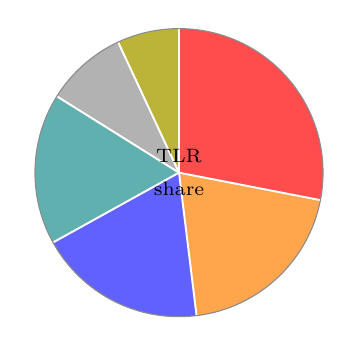
\begin{tikzpicture}[scale=1.18]
\def\r{1.55}
\fill[red!70] (0,0) -- (90:\r) arc (90:-11:\r) -- cycle;
\fill[orange!70] (0,0) -- (-11:\r) arc (-11:-83:\r) -- cycle;
\fill[blue!62] (0,0) -- (-83:\r) arc (-83:-151:\r) -- cycle;
\fill[teal!62] (0,0) -- (-151:\r) arc (-151:-212:\r) -- cycle;
\fill[gray!60] (0,0) -- (-212:\r) arc (-212:-245:\r) -- cycle;
\fill[yellow!70!black] (0,0) -- (-245:\r) arc (-245:-270:\r) -- cycle;
\draw[white,line width=0.7pt] (0,0) -- (90:\r);
\draw[white,line width=0.7pt] (0,0) -- (-11:\r);
\draw[white,line width=0.7pt] (0,0) -- (-83:\r);
\draw[white,line width=0.7pt] (0,0) -- (-151:\r);
\draw[white,line width=0.7pt] (0,0) -- (-212:\r);
\draw[white,line width=0.7pt] (0,0) -- (-245:\r);
\draw[white,line width=0.7pt] (0,0) -- (-270:\r);
\draw[black!45,line width=0.4pt] (0,0) circle (\r);
\node[align=center] at (0,0) {\scriptsize TLR\\\scriptsize share};
\end{tikzpicture}
\end{minipage}
\hfill
\begin{minipage}{0.58\textwidth}
\scriptsize
\begin{tabularx}{\linewidth}{L{0.08\linewidth} L{0.20\linewidth} Y}
\toprule
\textbf{Share} & \textbf{TLR bucket} & \textbf{Included faults} \\
\midrule
\textcolor{red!70}{28\%} & Security & Generated-code flaws, secrets, prompt injection, excessive agency, supply chain. \\
\textcolor{orange!80!black}{20\%} & Business truth & False-green business logic, authorization drift, data isolation. \\
\textcolor{blue!70}{19\%} & Verification & False-green tests, pixel/UI, accessibility, proof quality. \\
\textcolor{teal!70!black}{17\%} & Contracts/data & Contract drift, wrong-layer persistence, generated mutation. \\
\textcolor{gray!70}{9\%} & Context/setup & Context retrieval, setup hallucination, instruction drift. \\
\textcolor{yellow!60!black}{7\%} & Entropy & Dead language, mega files/functions, performance drift. \\
\bottomrule
\end{tabularx}
\end{minipage}
\caption{TLR means Top-Level Risk. Shares are derived from the taxonomy's policy-weighted RPN buckets for humanlint 0.2.0; they are not incident-frequency measurements. The chart is intended to steer audit priority: security and business truth receive first repair attention even when easier style findings are more numerous.}
\label{fig:tlr-pie}
\end{figure*}

\begin{center}
\fbox{\begin{minipage}{0.93\columnwidth}
\textbf{Highest-priority controls.} A humanlint-conformant repo should block merges when a changed path has no proof lane, a public boundary has handwritten contract mirrors, durable truth moves outside Rust/PostgreSQL ownership, security or secret scans are absent for risky changes, agent permissions are broader than the lane requires, user-facing UI lacks rendered proof, or \texttt{fallback}/\texttt{TODO}/\texttt{stub} ships without a scoped exception.
\end{minipage}}
\end{center}

The taxonomy turns insult into audit surface. A finding is useful only when it names the rule, points at exact evidence, gives a bounded repair, and can be serialized into an agent queue. ``This feels messy'' is not actionable. \texttt{HLT-002-GENERATED-MUTATION} in \texttt{apps/web/src/generated/client.ts} with source \texttt{contracts/openapi/api.yaml} is actionable.
